\SourceLeaf{354}

Soll nun
\[
A^2 + B^2 = -C^2
\]
sein, so werden wir haben:
\[\begin{aligned}
A &= (m+m'i)^2 - (n+n'i)^2 \\
B &= 2(m+m'i)(n+n'i) \\
C &= (m+m'i)^2 i + (n+n'i)^2 i.
\end{aligned}\]

Führt man diess aus, so ist:
\[\begin{aligned}
(m+m'i)^2 &= m^2 - m'^2 + 2mm'i \\
(n+n'i)^2 &= n^2 - n'^2 + 2nn'i \\
(m+m'i)(n+n'i) &= mn - m'n' + i(m'n+n'm),
\end{aligned}\]
also:
\[\begin{aligned}
A &= m^2 - m'^2 - n^2 + n'^2 + 2i(mm' - nn') \\
B &= 2(mn - m'n') + 2i(m'n+n'm) \\
C &= -2(mm'+nn') + i(m^2+n^2-m'^2-n'^2).
\end{aligned}\]

Umgekehrt kann man auch von diesen Zahlen auf die reellen zurückkommen.

Ist hier $m = 2$, $n = 1$, $m' = 1$, $n' = 1$, so erhält man:
\[
\begin{array}{lcl}
A = & 3+2i & \\
B = & 2+6i & \qquad A^2+B^2+C^2 = \left\{\begin{array}{r} 5+12i \\ -32+24i \\ +27-36i \end{array}\right\} = 0. \\
C = & -6+3i &
\end{array}
\]

\textls{Zusatz.} Sind die complexen Zahlen für die Ecken 1, 2, 3 gefunden, so hat man auch die für
die andern 4. Es sind nemlich die für:
\begin{center}\begin{minipage}{3.3cm}\[
\begin{array}{cc}
0 & 0 \\
1 & A \\
2 & B \\
3 & C \\
6 & A+B \\
7 & A+C \\
5 & A+B+C \\
4 & B+C
\end{array}
\]

\end{minipage}\hspace{.4cm}\begin{minipage}{7.1cm}\resizebox{7.1cm}{!}{%
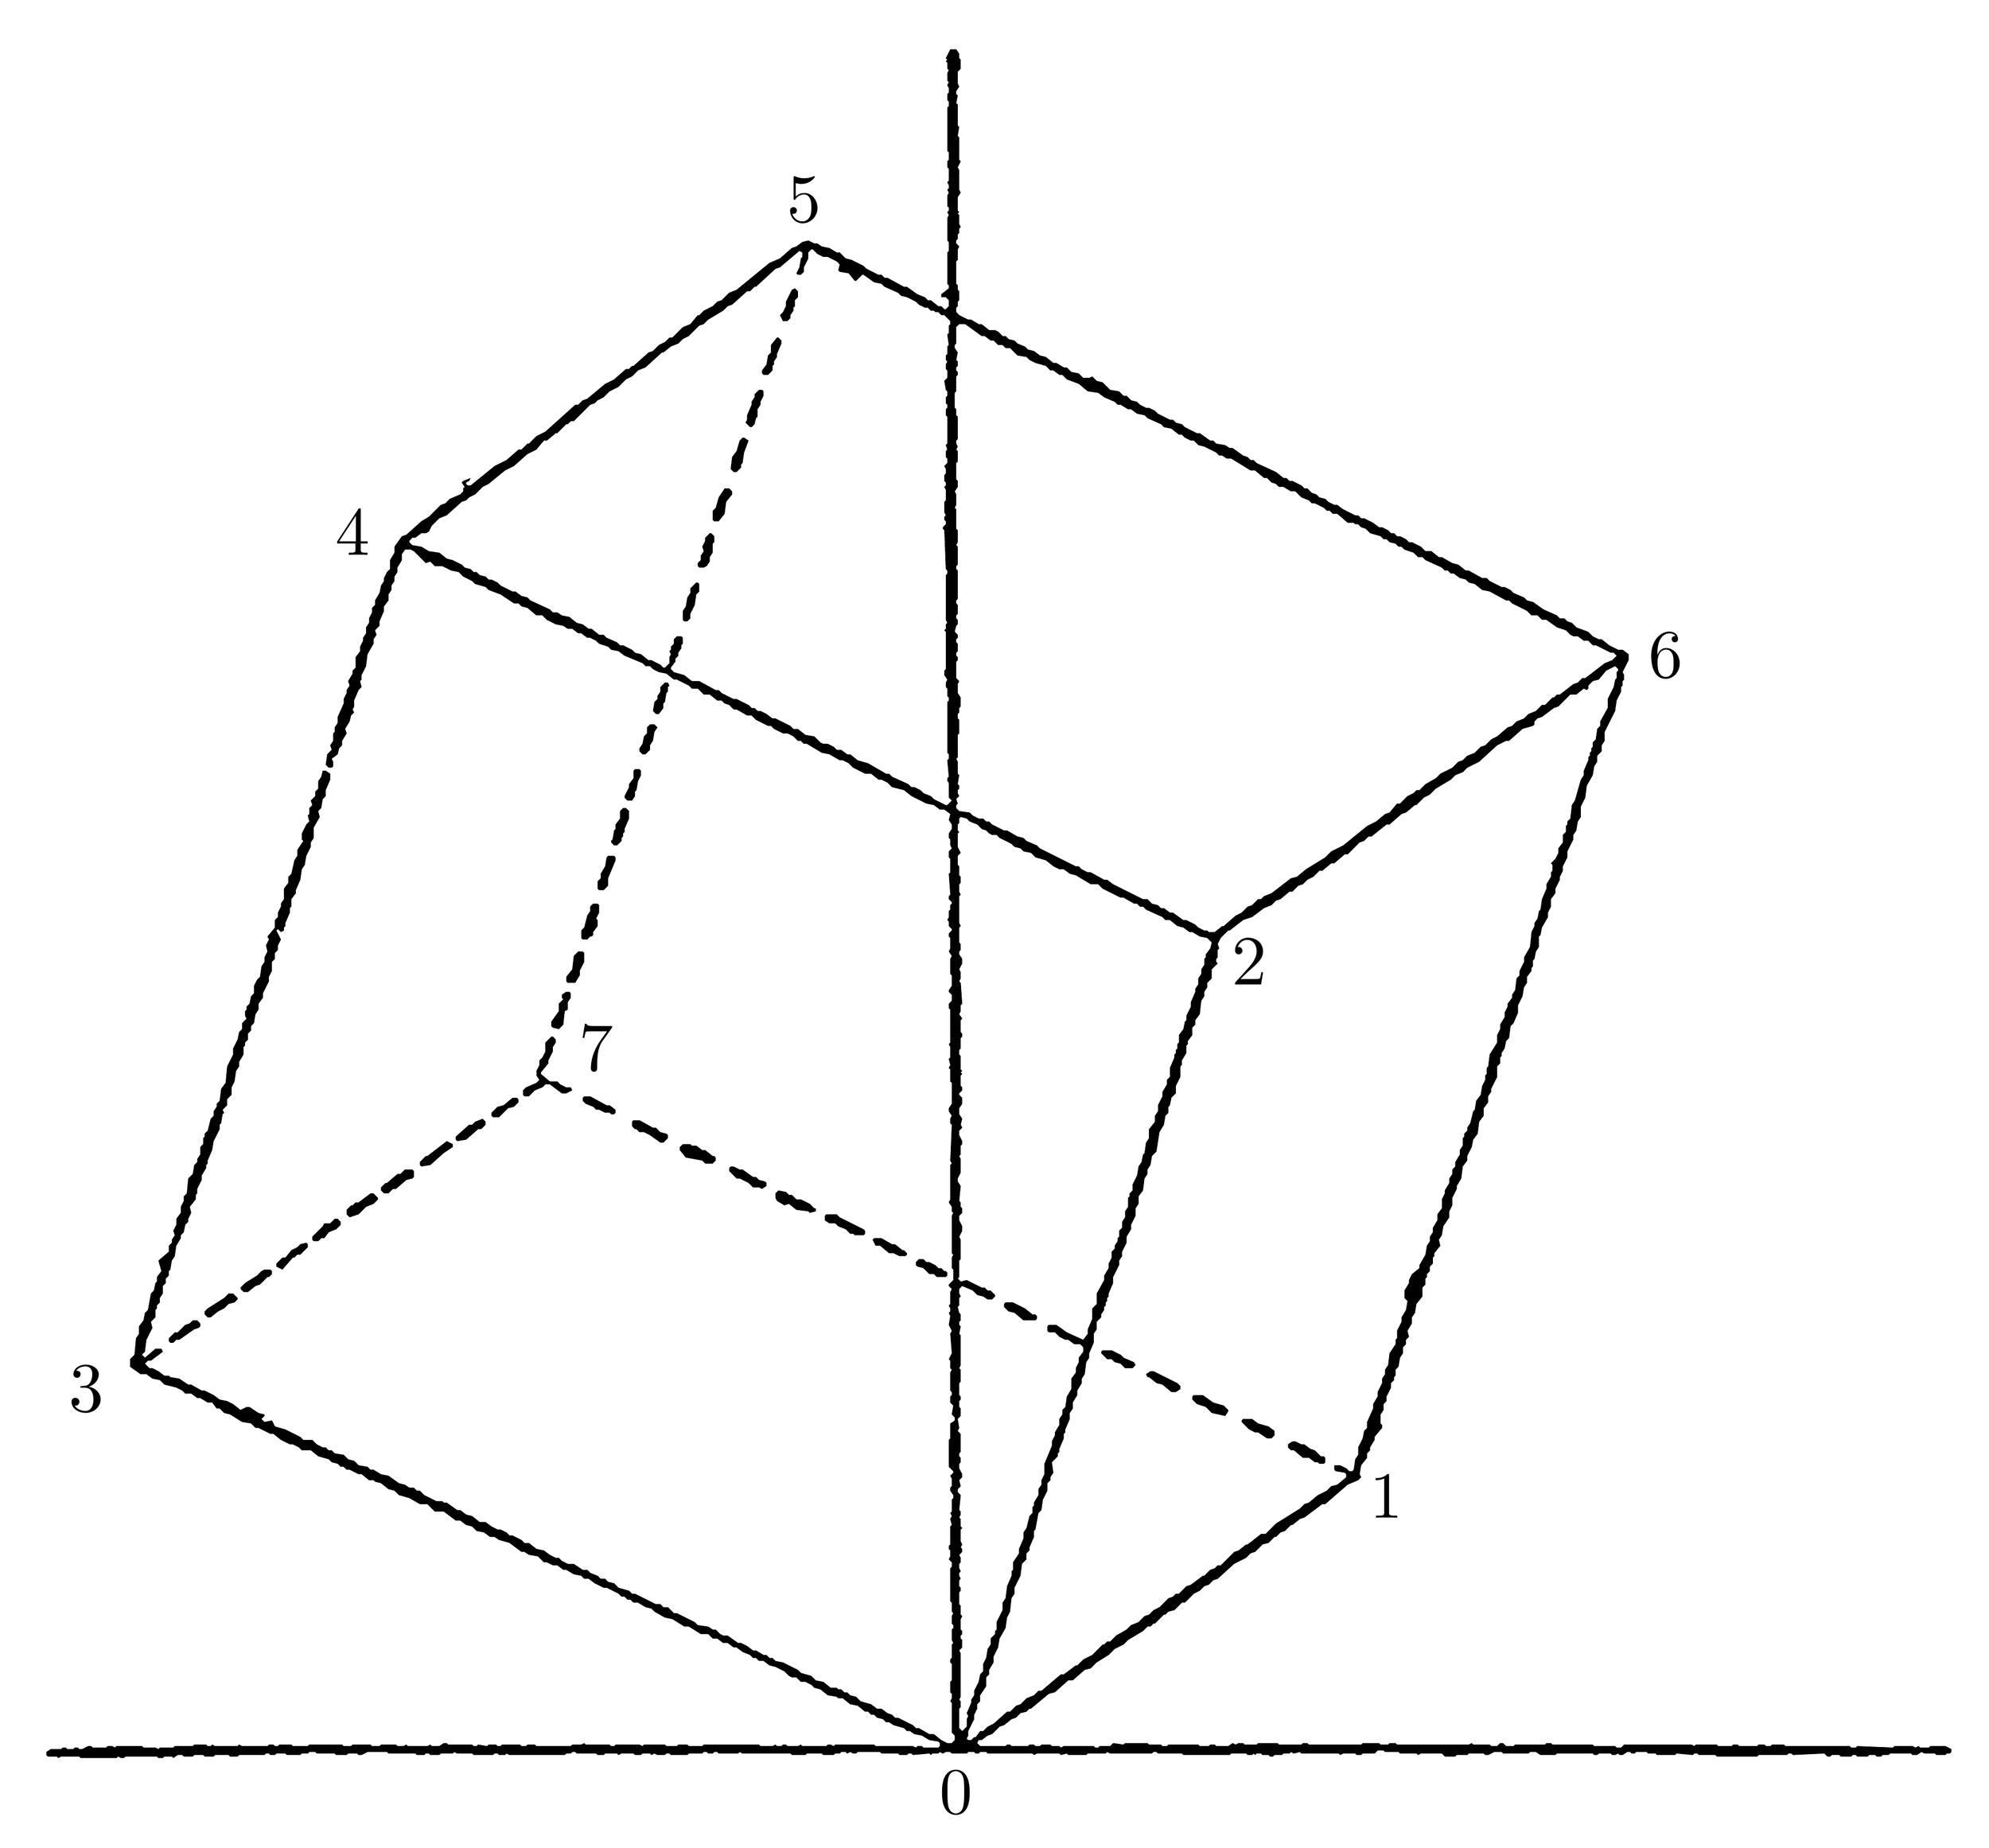
\begin{tikzpicture}[x=1pt,y=-1pt]
\path[use as bounding box] (0,0) rectangle (1311,1217);
\path[fill=black,draw=none,even odd rule]
(124,876) -- (122,874) -- (119,874) -- (117,876) -- (114,877) -- (109,882) -- (107,882) -- (103,886) -- (103,888) -- (104,889) -- (106,889) -- (108,887) -- (110,887) -- (120,880) -- (123,879) -- (124,878) -- cycle
(149,859) -- (146,856) -- (143,856) -- (140,859) -- (129,866) -- (127,868) -- (127,870) -- (129,872) -- (131,872) -- (136,868) -- (140,866) -- (143,863) -- (147,862) -- (149,860) -- cycle
(172,841) -- (171,840) -- (167,840) -- (165,841) -- (162,844) -- (154,849) -- (151,852) -- (151,853) -- (153,855) -- (156,855) -- (161,851) -- (164,850) -- (169,845) -- (170,845) -- (172,843) -- cycle
(603,835) -- (603,837) -- (604,838) -- (608,839) -- (612,843) -- (615,843) -- (617,845) -- (623,845) -- (624,844) -- (624,842) -- (623,841) -- (622,841) -- (620,839) -- (618,839) -- (616,837) -- (612,835) -- (610,835) -- (608,833) -- (605,833) -- cycle
(196,823) -- (195,822) -- (191,823) -- (189,825) -- (185,827) -- (181,832) -- (179,832) -- (175,836) -- (175,838) -- (179,840) -- (186,832) -- (187,832) -- (189,830) -- (191,830) -- (196,825) -- cycle
(574,820) -- (576,824) -- (579,824) -- (585,829) -- (588,829) -- (592,831) -- (596,831) -- (597,830) -- (597,829) -- (595,827) -- (594,827) -- (589,823) -- (587,823) -- (580,819) -- (575,819) -- cycle
(218,808) -- (216,806) -- (214,806) -- (211,809) -- (207,809) -- (206,811) -- (199,818) -- (199,820) -- (200,821) -- (203,821) -- (205,819) -- (207,819) -- (210,815) -- (215,813) -- (218,810) -- cycle
(542,804) -- (542,807) -- (545,809) -- (549,809) -- (551,811) -- (556,813) -- (559,816) -- (561,816) -- (562,817) -- (568,817) -- (569,816) -- (569,814) -- (568,813) -- (552,805) -- (550,803) -- (543,803) -- cycle
(243,792) -- (240,789) -- (238,789) -- (230,795) -- (228,795) -- (226,797) -- (225,797) -- (222,800) -- (222,803) -- (224,805) -- (230,803) -- (235,798) -- (240,796) -- (243,793) -- cycle
(509,789) -- (509,792) -- (510,794) -- (515,797) -- (518,796) -- (523,800) -- (531,801) -- (532,802) -- (536,801) -- (536,799) -- (535,799) -- (532,796) -- (526,793) -- (523,793) -- (520,790) -- (518,790) -- (516,788) -- (511,787) -- cycle
(267,774) -- (266,773) -- (261,773) -- (258,776) -- (256,776) -- (249,782) -- (248,782) -- (245,785) -- (245,787) -- (247,789) -- (250,789) -- (253,786) -- (255,786) -- (262,780) -- (266,779) -- (267,778) -- cycle
(478,772) -- (478,774) -- (483,779) -- (485,779) -- (491,782) -- (494,785) -- (498,785) -- (500,786) -- (503,784) -- (503,782) -- (502,781) -- (498,780) -- (496,778) -- (494,778) -- (487,773) -- (485,773) -- (481,771) -- (479,771) -- cycle
(445,758) -- (445,760) -- (449,765) -- (460,767) -- (462,769) -- (467,769) -- (469,767) -- (469,765) -- (468,764) -- (467,764) -- (462,760) -- (460,760) -- (456,757) -- (453,757) -- (452,756) -- (447,756) -- cycle
(293,756) -- (289,754) -- (276,764) -- (275,764) -- (271,768) -- (271,770) -- (272,771) -- (278,770) -- (287,762) -- (293,758) -- cycle
(413,741) -- (413,744) -- (415,746) -- (416,746) -- (418,748) -- (421,748) -- (425,750) -- (432,755) -- (434,755) -- (437,752) -- (437,750) -- (436,749) -- (432,748) -- (429,745) -- (427,745) -- (418,740) -- (414,740) -- cycle
(315,741) -- (313,739) -- (308,741) -- (306,743) -- (304,743) -- (295,751) -- (295,753) -- (296,754) -- (302,753) -- (310,746) -- (312,746) -- (315,743) -- cycle
(337,726) -- (336,725) -- (333,725) -- (327,730) -- (323,731) -- (319,735) -- (319,737) -- (320,738) -- (324,738) -- (330,732) -- (334,731) -- (337,728) -- cycle
(380,725) -- (380,727) -- (382,729) -- (387,731) -- (389,733) -- (391,733) -- (395,735) -- (398,735) -- (399,736) -- (401,736) -- (402,735) -- (402,733) -- (398,730) -- (396,730) -- (385,724) -- (381,724) -- cycle
(360,684) -- (359,684) -- (355,688) -- (355,694) -- (353,698) -- (351,700) -- (351,703) -- (349,707) -- (349,710) -- (351,713) -- (349,715) -- (342,718) -- (340,720) -- (340,723) -- (341,724) -- (344,724) -- (348,720) -- (353,718) -- (355,716) -- (358,716) -- (366,722) -- (369,722) -- (373,720) -- (372,718) -- (369,718) -- (365,716) -- (363,714) -- (358,714) -- (352,709) -- (352,708) -- (357,702) -- (357,700) -- (360,694) -- (360,691) -- (362,688) -- (362,686) -- cycle
(371,654) -- (369,654) -- (366,656) -- (366,658) -- (367,659) -- (364,662) -- (364,667) -- (359,674) -- (359,677) -- (360,678) -- (364,679) -- (367,676) -- (368,667) -- (370,666) -- (370,661) -- (372,658) -- (372,655) -- cycle
(380,627) -- (377,627) -- (374,630) -- (373,639) -- (369,644) -- (369,647) -- (370,648) -- (375,648) -- (378,643) -- (378,640) -- (381,634) -- (381,628) -- cycle
(390,595) -- (387,595) -- (385,597) -- (385,600) -- (383,603) -- (381,611) -- (379,613) -- (379,618) -- (380,619) -- (383,619) -- (385,617) -- (386,617) -- (387,616) -- (387,614) -- (390,610) -- (390,606) -- (389,605) -- (391,601) -- (391,596) -- cycle
(401,563) -- (397,563) -- (396,564) -- (395,570) -- (392,575) -- (392,578) -- (390,580) -- (390,585) -- (391,586) -- (394,586) -- (397,583) -- (397,578) -- (402,566) -- (402,564) -- cycle
(409,531) -- (407,531) -- (405,533) -- (405,538) -- (402,542) -- (402,545) -- (401,546) -- (400,552) -- (399,553) -- (399,554) -- (401,556) -- (403,556) -- (406,553) -- (406,551) -- (407,550) -- (407,548) -- (408,547) -- (408,545) -- (411,538) -- (411,533) -- cycle
(418,505) -- (415,505) -- (414,506) -- (414,511) -- (411,515) -- (411,517) -- (408,523) -- (408,524) -- (410,526) -- (413,526) -- (415,523) -- (415,520) -- (416,519) -- (417,513) -- (419,509) -- (419,506) -- cycle
(428,475) -- (425,475) -- (423,477) -- (423,481) -- (421,483) -- (420,488) -- (418,491) -- (418,493) -- (420,495) -- (422,495) -- (425,492) -- (425,489) -- (427,486) -- (428,480) -- (430,477) -- cycle
(437,447) -- (435,447) -- (432,450) -- (432,453) -- (430,456) -- (430,458) -- (428,460) -- (427,466) -- (429,468) -- (431,468) -- (434,464) -- (434,461) -- (435,460) -- (436,454) -- (437,453) -- (437,450) -- (438,449) -- cycle
(626,23) -- (623,29) -- (624,30) -- (623,31) -- (624,32) -- (624,36) -- (625,37) -- (624,39) -- (624,44) -- (625,45) -- (624,47) -- (625,49) -- (625,52) -- (624,53) -- (624,57) -- (625,58) -- (625,61) -- (624,62) -- (624,91) -- (625,92) -- (625,97) -- (624,98) -- (624,102) -- (625,103) -- (625,111) -- (624,112) -- (625,114) -- (625,116) -- (624,117) -- (625,119) -- (624,121) -- (624,128) -- (625,129) -- (625,131) -- (624,132) -- (625,134) -- (624,136) -- (624,151) -- (625,152) -- (625,158) -- (624,159) -- (624,180) -- (625,181) -- (625,183) -- (620,187) -- (620,189) -- (623,189) -- (625,191) -- (625,195) -- (623,197) -- (622,197) -- (620,195) -- (618,195) -- (613,191) -- (611,191) -- (609,189) -- (604,187) -- (597,182) -- (595,182) -- (584,176) -- (582,176) -- (580,174) -- (578,174) -- (570,170) -- (568,168) -- (560,164) -- (556,163) -- (552,159) -- (550,159) -- (545,156) -- (540,155) -- (537,153) -- (535,153) -- (531,151) -- (527,152) -- (523,155) -- (520,156) -- (512,163) -- (505,166) -- (483,184) -- (478,186) -- (473,191) -- (470,192) -- (467,195) -- (461,198) -- (458,201) -- (457,201) -- (452,207) -- (447,209) -- (440,216) -- (438,216) -- (435,219) -- (431,221) -- (427,225) -- (424,226) -- (414,235) -- (413,235) -- (411,237) -- (409,237) -- (401,244) -- (395,247) -- (383,257) -- (380,258) -- (377,261) -- (375,261) -- (355,279) -- (349,282) -- (344,287) -- (343,287) -- (339,291) -- (337,291) -- (329,298) -- (321,302) -- (305,315) -- (303,315) -- (302,314) -- (302,313) -- (304,312) -- (305,310) -- (300,312) -- (299,313) -- (301,316) -- (300,317) -- (300,319) -- (298,321) -- (291,324) -- (288,327) -- (285,328) -- (277,336) -- (272,339) -- (262,348) -- (259,349) -- (254,356) -- (254,360) -- (251,365) -- (251,371) -- (249,373) -- (247,377) -- (247,379) -- (245,382) -- (244,387) -- (241,392) -- (241,395) -- (239,397) -- (239,400) -- (237,404) -- (237,407) -- (235,410) -- (235,414) -- (233,417) -- (233,419) -- (231,423) -- (231,426) -- (228,430) -- (228,437) -- (226,439) -- (226,441) -- (223,446) -- (224,449) -- (222,452) -- (222,454) -- (220,458) -- (220,461) -- (216,470) -- (216,474) -- (214,477) -- (214,480) -- (213,481) -- (213,486) -- (211,489) -- (212,492) -- (209,495) -- (208,502) -- (210,504) -- (212,504) -- (213,503) -- (213,500) -- (212,498) -- (216,495) -- (217,491) -- (219,489) -- (219,486) -- (222,481) -- (221,478) -- (224,473) -- (225,469) -- (227,467) -- (226,465) -- (227,463) -- (227,459) -- (230,452) -- (232,450) -- (231,446) -- (232,445) -- (232,442) -- (235,436) -- (236,428) -- (240,421) -- (240,418) -- (242,415) -- (241,412) -- (244,409) -- (244,406) -- (247,399) -- (247,396) -- (250,392) -- (250,388) -- (252,385) -- (252,382) -- (254,379) -- (254,376) -- (256,373) -- (256,370) -- (259,365) -- (259,361) -- (261,358) -- (265,358) -- (267,359) -- (275,367) -- (278,366) -- (281,369) -- (286,369) -- (292,372) -- (297,373) -- (300,376) -- (306,379) -- (308,381) -- (315,383) -- (317,385) -- (325,388) -- (334,394) -- (337,394) -- (339,396) -- (343,397) -- (349,402) -- (353,402) -- (356,405) -- (362,408) -- (367,409) -- (370,411) -- (373,411) -- (377,414) -- (379,414) -- (383,417) -- (385,417) -- (389,419) -- (391,421) -- (397,423) -- (399,425) -- (404,426) -- (408,429) -- (420,434) -- (422,436) -- (425,436) -- (427,438) -- (431,440) -- (436,441) -- (441,445) -- (443,445) -- (451,449) -- (453,451) -- (457,451) -- (461,455) -- (465,455) -- (470,459) -- (473,459) -- (475,461) -- (478,462) -- (481,465) -- (483,465) -- (490,469) -- (493,469) -- (496,472) -- (504,476) -- (506,476) -- (508,478) -- (514,481) -- (517,481) -- (521,483) -- (524,486) -- (526,486) -- (528,488) -- (530,488) -- (540,494) -- (545,495) -- (552,499) -- (554,499) -- (558,501) -- (561,504) -- (569,508) -- (573,508) -- (578,512) -- (580,512) -- (584,514) -- (587,517) -- (595,519) -- (600,523) -- (610,528) -- (615,529) -- (619,532) -- (622,532) -- (626,535) -- (625,539) -- (627,542) -- (627,545) -- (625,548) -- (625,551) -- (626,552) -- (626,556) -- (627,558) -- (625,560) -- (625,564) -- (626,565) -- (626,574) -- (625,575) -- (626,589) -- (625,590) -- (625,592) -- (627,594) -- (627,595) -- (626,596) -- (626,599) -- (625,600) -- (625,604) -- (624,606) -- (625,607) -- (625,610) -- (627,612) -- (627,613) -- (625,615) -- (625,617) -- (626,618) -- (626,625) -- (625,627) -- (627,630) -- (626,632) -- (626,642) -- (627,643) -- (627,650) -- (625,653) -- (625,654) -- (627,656) -- (627,660) -- (625,662) -- (625,665) -- (626,666) -- (626,688) -- (625,689) -- (626,691) -- (626,698) -- (625,699) -- (626,703) -- (625,705) -- (626,706) -- (626,714) -- (627,715) -- (627,729) -- (625,732) -- (625,734) -- (627,737) -- (626,739) -- (626,742) -- (627,743) -- (626,767) -- (627,769) -- (626,770) -- (626,793) -- (625,795) -- (627,798) -- (627,801) -- (628,802) -- (627,804) -- (627,829) -- (628,830) -- (627,832) -- (627,839) -- (628,840) -- (628,847) -- (625,850) -- (625,851) -- (627,853) -- (626,855) -- (626,863) -- (625,864) -- (626,866) -- (626,868) -- (625,869) -- (626,871) -- (625,877) -- (627,881) -- (626,883) -- (627,896) -- (625,900) -- (626,901) -- (626,906) -- (627,907) -- (626,909) -- (626,921) -- (627,922) -- (627,924) -- (626,925) -- (626,929) -- (628,931) -- (627,937) -- (629,939) -- (629,941) -- (626,943) -- (626,953) -- (625,954) -- (625,972) -- (628,975) -- (628,976) -- (626,978) -- (627,980) -- (627,985) -- (626,986) -- (626,988) -- (628,991) -- (628,993) -- (627,994) -- (627,1002) -- (626,1003) -- (627,1005) -- (626,1007) -- (627,1011) -- (626,1012) -- (626,1024) -- (625,1025) -- (625,1027) -- (626,1028) -- (626,1032) -- (625,1034) -- (627,1036) -- (627,1039) -- (626,1040) -- (626,1062) -- (627,1063) -- (627,1069) -- (628,1070) -- (627,1072) -- (627,1077) -- (628,1078) -- (628,1080) -- (627,1081) -- (627,1088) -- (628,1090) -- (627,1091) -- (627,1100) -- (626,1101) -- (626,1103) -- (627,1104) -- (627,1115) -- (626,1116) -- (626,1123) -- (627,1124) -- (627,1127) -- (626,1129) -- (627,1130) -- (627,1150) -- (629,1152) -- (629,1155) -- (627,1157) -- (624,1157) -- (620,1155) -- (615,1151) -- (612,1151) -- (605,1147) -- (603,1147) -- (601,1145) -- (591,1140) -- (589,1140) -- (587,1138) -- (584,1137) -- (580,1134) -- (577,1134) -- (573,1131) -- (566,1129) -- (563,1126) -- (559,1125) -- (557,1123) -- (555,1123) -- (553,1121) -- (551,1121) -- (550,1120) -- (546,1120) -- (541,1116) -- (536,1115) -- (533,1112) -- (526,1110) -- (524,1108) -- (514,1103) -- (509,1102) -- (507,1100) -- (505,1100) -- (503,1098) -- (501,1098) -- (496,1095) -- (494,1095) -- (490,1092) -- (486,1090) -- (484,1090) -- (477,1085) -- (474,1085) -- (472,1084) -- (469,1081) -- (467,1081) -- (464,1079) -- (457,1078) -- (455,1076) -- (443,1070) -- (441,1070) -- (437,1066) -- (434,1066) -- (432,1064) -- (429,1064) -- (415,1057) -- (413,1057) -- (411,1055) -- (404,1053) -- (401,1050) -- (397,1049) -- (395,1047) -- (392,1047) -- (390,1045) -- (385,1043) -- (383,1041) -- (380,1041) -- (374,1037) -- (370,1037) -- (366,1035) -- (364,1033) -- (362,1033) -- (358,1031) -- (354,1028) -- (349,1027) -- (344,1023) -- (341,1023) -- (339,1021) -- (333,1018) -- (331,1018) -- (329,1016) -- (325,1014) -- (323,1014) -- (319,1012) -- (315,1009) -- (311,1009) -- (306,1005) -- (302,1004) -- (298,1001) -- (296,1001) -- (289,996) -- (287,996) -- (286,995) -- (282,995) -- (274,991) -- (271,988) -- (269,988) -- (267,986) -- (264,986) -- (261,984) -- (257,983) -- (250,978) -- (245,977) -- (240,974) -- (238,974) -- (236,972) -- (230,971) -- (227,968) -- (223,967) -- (220,964) -- (214,963) -- (212,961) -- (210,961) -- (208,959) -- (206,959) -- (202,957) -- (199,954) -- (193,954) -- (191,952) -- (181,947) -- (174,945) -- (172,941) -- (167,942) -- (165,940) -- (167,938) -- (167,937) -- (163,936) -- (157,932) -- (155,932) -- (151,934) -- (146,930) -- (142,928) -- (137,927) -- (133,924) -- (127,921) -- (125,921) -- (118,917) -- (116,917) -- (110,913) -- (104,912) -- (103,911) -- (100,911) -- (96,908) -- (92,906) -- (90,906) -- (87,903) -- (89,901) -- (91,901) -- (99,895) -- (98,893) -- (94,893) -- (87,899) -- (85,897) -- (87,895) -- (88,887) -- (92,879) -- (91,875) -- (94,872) -- (94,867) -- (95,866) -- (95,864) -- (97,862) -- (97,859) -- (99,856) -- (99,851) -- (101,849) -- (101,846) -- (103,844) -- (103,841) -- (104,840) -- (105,834) -- (107,831) -- (108,824) -- (111,819) -- (111,817) -- (113,815) -- (114,810) -- (116,808) -- (116,806) -- (118,802) -- (117,798) -- (121,793) -- (121,790) -- (122,789) -- (122,786) -- (125,780) -- (125,777) -- (128,772) -- (128,770) -- (129,769) -- (129,767) -- (132,760) -- (133,754) -- (137,746) -- (137,743) -- (138,742) -- (139,736) -- (140,735) -- (139,733) -- (142,730) -- (142,726) -- (145,723) -- (145,718) -- (147,714) -- (148,707) -- (150,704) -- (150,701) -- (153,696) -- (153,691) -- (154,690) -- (154,688) -- (156,686) -- (156,682) -- (158,680) -- (158,677) -- (160,675) -- (161,669) -- (163,666) -- (163,662) -- (166,658) -- (166,655) -- (170,647) -- (170,644) -- (172,640) -- (172,634) -- (174,632) -- (174,628) -- (176,626) -- (176,623) -- (178,619) -- (175,613) -- (176,612) -- (178,614) -- (180,613) -- (180,611) -- (181,610) -- (181,608) -- (184,601) -- (184,598) -- (185,597) -- (185,592) -- (188,588) -- (188,586) -- (191,579) -- (192,572) -- (194,569) -- (195,563) -- (198,557) -- (198,554) -- (200,551) -- (200,544) -- (204,537) -- (203,533) -- (205,531) -- (206,525) -- (208,523) -- (208,519) -- (211,512) -- (211,508) -- (208,506) -- (206,506) -- (205,510) -- (203,513) -- (203,518) -- (201,520) -- (201,523) -- (198,526) -- (199,529) -- (197,531) -- (197,535) -- (196,536) -- (197,540) -- (195,542) -- (192,548) -- (192,552) -- (193,553) -- (189,559) -- (189,563) -- (187,566) -- (185,575) -- (183,577) -- (183,581) -- (180,585) -- (180,592) -- (178,595) -- (178,597) -- (176,601) -- (176,604) -- (174,606) -- (174,611) -- (169,617) -- (170,619) -- (168,623) -- (169,627) -- (167,631) -- (167,634) -- (165,637) -- (164,644) -- (162,646) -- (160,650) -- (160,655) -- (158,657) -- (157,662) -- (155,664) -- (155,666) -- (154,667) -- (154,670) -- (155,672) -- (152,675) -- (152,679) -- (150,681) -- (149,686) -- (146,692) -- (146,696) -- (142,704) -- (141,715) -- (138,719) -- (137,727) -- (135,729) -- (135,731) -- (133,734) -- (133,737) -- (131,739) -- (129,747) -- (127,749) -- (127,751) -- (126,752) -- (126,756) -- (124,758) -- (124,763) -- (122,766) -- (122,768) -- (120,770) -- (119,776) -- (116,779) -- (115,789) -- (113,791) -- (113,794) -- (111,798) -- (111,802) -- (108,806) -- (108,810) -- (106,814) -- (107,817) -- (105,820) -- (105,822) -- (103,824) -- (103,828) -- (96,834) -- (98,841) -- (95,845) -- (95,848) -- (94,849) -- (93,854) -- (91,856) -- (89,867) -- (87,869) -- (86,874) -- (83,878) -- (83,883) -- (81,886) -- (80,897) -- (77,900) -- (77,905) -- (84,910) -- (88,910) -- (92,913) -- (97,914) -- (100,917) -- (108,919) -- (112,921) -- (114,923) -- (118,923) -- (122,926) -- (124,926) -- (129,929) -- (132,929) -- (135,933) -- (137,933) -- (140,936) -- (144,937) -- (152,942) -- (158,943) -- (161,946) -- (163,946) -- (171,950) -- (173,950) -- (178,954) -- (184,957) -- (186,957) -- (190,959) -- (192,961) -- (198,961) -- (203,965) -- (210,967) -- (212,969) -- (216,970) -- (218,972) -- (220,972) -- (222,974) -- (224,974) -- (230,977) -- (232,977) -- (237,981) -- (240,981) -- (241,982) -- (245,983) -- (250,987) -- (254,988) -- (257,991) -- (264,993) -- (271,997) -- (276,997) -- (281,1002) -- (287,1002) -- (295,1008) -- (298,1008) -- (302,1011) -- (306,1012) -- (309,1015) -- (314,1016) -- (318,1019) -- (321,1019) -- (324,1021) -- (331,1023) -- (339,1029) -- (341,1029) -- (344,1031) -- (350,1032) -- (354,1036) -- (356,1036) -- (360,1038) -- (363,1038) -- (367,1041) -- (369,1041) -- (374,1044) -- (379,1045) -- (381,1047) -- (384,1047) -- (388,1050) -- (394,1053) -- (396,1053) -- (404,1057) -- (406,1059) -- (408,1059) -- (410,1061) -- (412,1061) -- (414,1063) -- (417,1063) -- (422,1066) -- (426,1067) -- (428,1069) -- (435,1073) -- (440,1074) -- (448,1079) -- (451,1079) -- (459,1084) -- (464,1084) -- (467,1087) -- (470,1087) -- (474,1090) -- (477,1090) -- (481,1093) -- (483,1093) -- (487,1096) -- (492,1098) -- (494,1100) -- (496,1100) -- (498,1102) -- (501,1102) -- (505,1105) -- (509,1106) -- (515,1109) -- (518,1112) -- (520,1113) -- (523,1113) -- (526,1116) -- (529,1116) -- (533,1118) -- (535,1120) -- (539,1121) -- (544,1125) -- (550,1126) -- (551,1127) -- (554,1127) -- (559,1131) -- (564,1132) -- (569,1136) -- (571,1136) -- (573,1138) -- (575,1138) -- (577,1140) -- (581,1141) -- (583,1143) -- (585,1143) -- (588,1145) -- (595,1147) -- (597,1149) -- (599,1149) -- (602,1151) -- (607,1152) -- (612,1155) -- (618,1156) -- (619,1157) -- (619,1159) -- (618,1160) -- (608,1160) -- (607,1159) -- (604,1159) -- (603,1160) -- (601,1159) -- (576,1159) -- (575,1158) -- (549,1158) -- (548,1159) -- (546,1158) -- (544,1158) -- (543,1159) -- (527,1159) -- (526,1158) -- (524,1159) -- (517,1159) -- (516,1158) -- (514,1158) -- (513,1159) -- (510,1159) -- (509,1158) -- (507,1159) -- (499,1159) -- (498,1158) -- (461,1158) -- (460,1159) -- (451,1159) -- (450,1158) -- (444,1158) -- (443,1159) -- (436,1159) -- (435,1158) -- (421,1158) -- (420,1159) -- (418,1158) -- (402,1158) -- (401,1159) -- (399,1159) -- (398,1158) -- (382,1158) -- (381,1157) -- (379,1158) -- (373,1158) -- (372,1159) -- (349,1159) -- (348,1158) -- (343,1158) -- (342,1159) -- (339,1159) -- (338,1158) -- (326,1158) -- (325,1159) -- (323,1159) -- (322,1158) -- (317,1158) -- (316,1159) -- (310,1158) -- (309,1159) -- (307,1159) -- (306,1158) -- (290,1158) -- (289,1157) -- (287,1157) -- (284,1159) -- (279,1159) -- (278,1158) -- (276,1159) -- (263,1159) -- (262,1158) -- (260,1159) -- (256,1159) -- (255,1158) -- (245,1158) -- (244,1159) -- (239,1159) -- (238,1158) -- (226,1158) -- (225,1159) -- (220,1159) -- (219,1158) -- (197,1158) -- (196,1159) -- (186,1159) -- (185,1158) -- (177,1158) -- (176,1159) -- (174,1159) -- (173,1158) -- (170,1158) -- (169,1159) -- (152,1159) -- (150,1158) -- (149,1159) -- (134,1159) -- (132,1158) -- (131,1159) -- (129,1159) -- (128,1158) -- (120,1158) -- (119,1159) -- (107,1159) -- (106,1160) -- (97,1160) -- (96,1161) -- (94,1160) -- (86,1160) -- (85,1159) -- (68,1159) -- (67,1160) -- (65,1159) -- (62,1159) -- (61,1160) -- (52,1160) -- (51,1159) -- (49,1159) -- (45,1161) -- (43,1161) -- (42,1160) -- (40,1160) -- (39,1161) -- (35,1161) -- (34,1160) -- (32,1160) -- (31,1161) -- (24,1161) -- (21,1163) -- (21,1165) -- (22,1166) -- (28,1166) -- (29,1167) -- (31,1166) -- (43,1166) -- (44,1167) -- (68,1167) -- (69,1166) -- (71,1167) -- (73,1167) -- (74,1166) -- (95,1166) -- (96,1167) -- (99,1167) -- (100,1166) -- (105,1166) -- (106,1167) -- (109,1165) -- (112,1165) -- (113,1166) -- (119,1166) -- (120,1165) -- (126,1165) -- (127,1166) -- (133,1166) -- (134,1165) -- (143,1165) -- (144,1166) -- (149,1166) -- (150,1165) -- (167,1165) -- (168,1164) -- (170,1164) -- (171,1165) -- (174,1165) -- (175,1164) -- (181,1164) -- (182,1165) -- (191,1165) -- (192,1164) -- (196,1164) -- (197,1163) -- (201,1163) -- (202,1164) -- (214,1164) -- (215,1165) -- (222,1165) -- (223,1164) -- (229,1164) -- (230,1165) -- (232,1165) -- (236,1163) -- (249,1163) -- (250,1164) -- (268,1164) -- (269,1165) -- (274,1165) -- (275,1164) -- (277,1164) -- (278,1165) -- (284,1165) -- (285,1164) -- (293,1164) -- (294,1163) -- (296,1164) -- (306,1164) -- (307,1165) -- (320,1165) -- (321,1164) -- (323,1164) -- (324,1165) -- (328,1165) -- (329,1164) -- (331,1165) -- (368,1165) -- (369,1164) -- (372,1164) -- (373,1163) -- (375,1163) -- (376,1164) -- (389,1164) -- (390,1165) -- (394,1165) -- (395,1164) -- (403,1164) -- (404,1165) -- (406,1164) -- (414,1164) -- (415,1165) -- (419,1165) -- (420,1164) -- (425,1164) -- (426,1165) -- (428,1164) -- (430,1165) -- (435,1165) -- (436,1164) -- (438,1164) -- (439,1165) -- (450,1165) -- (451,1164) -- (460,1164) -- (461,1163) -- (463,1163) -- (464,1164) -- (467,1164) -- (468,1163) -- (470,1163) -- (471,1164) -- (484,1164) -- (485,1163) -- (487,1164) -- (519,1164) -- (520,1165) -- (529,1165) -- (530,1164) -- (540,1164) -- (541,1165) -- (548,1165) -- (549,1164) -- (552,1164) -- (553,1163) -- (556,1163) -- (557,1164) -- (559,1163) -- (561,1164) -- (563,1164) -- (564,1163) -- (579,1163) -- (580,1164) -- (591,1164) -- (592,1165) -- (597,1165) -- (598,1164) -- (600,1164) -- (601,1165) -- (612,1164) -- (613,1165) -- (614,1164) -- (618,1164) -- (619,1163) -- (621,1164) -- (623,1163) -- (626,1163) -- (627,1164) -- (637,1164) -- (638,1163) -- (642,1163) -- (643,1164) -- (645,1164) -- (646,1163) -- (650,1163) -- (651,1164) -- (681,1164) -- (682,1165) -- (684,1164) -- (699,1164) -- (700,1165) -- (704,1164) -- (705,1165) -- (717,1165) -- (718,1164) -- (730,1164) -- (731,1163) -- (733,1164) -- (761,1164) -- (762,1163) -- (764,1163) -- (765,1164) -- (781,1164) -- (782,1165) -- (813,1165) -- (814,1164) -- (824,1164) -- (825,1165) -- (828,1165) -- (829,1164) -- (830,1165) -- (831,1164) -- (834,1164) -- (835,1165) -- (839,1165) -- (840,1166) -- (842,1166) -- (843,1165) -- (848,1165) -- (849,1164) -- (853,1164) -- (854,1163) -- (856,1164) -- (860,1163) -- (861,1164) -- (886,1164) -- (887,1165) -- (889,1164) -- (897,1164) -- (898,1165) -- (901,1165) -- (902,1164) -- (910,1164) -- (912,1162) -- (916,1162) -- (917,1163) -- (926,1163) -- (927,1164) -- (938,1164) -- (939,1165) -- (941,1164) -- (955,1164) -- (957,1166) -- (964,1166) -- (965,1165) -- (972,1165) -- (973,1164) -- (983,1164) -- (984,1165) -- (986,1165) -- (990,1163) -- (995,1163) -- (996,1164) -- (1013,1164) -- (1014,1163) -- (1018,1163) -- (1021,1165) -- (1031,1165) -- (1032,1164) -- (1056,1164) -- (1057,1165) -- (1059,1165) -- (1060,1164) -- (1068,1164) -- (1069,1165) -- (1071,1165) -- (1073,1164) -- (1074,1165) -- (1076,1165) -- (1079,1163) -- (1081,1163) -- (1082,1164) -- (1084,1164) -- (1085,1163) -- (1092,1163) -- (1093,1164) -- (1098,1164) -- (1099,1165) -- (1111,1165) -- (1112,1164) -- (1123,1165) -- (1124,1164) -- (1126,1164) -- (1127,1165) -- (1138,1165) -- (1139,1166) -- (1166,1166) -- (1167,1165) -- (1186,1165) -- (1187,1164) -- (1189,1164) -- (1190,1165) -- (1211,1164) -- (1213,1166) -- (1215,1166) -- (1216,1165) -- (1221,1165) -- (1222,1166) -- (1229,1166) -- (1230,1165) -- (1232,1165) -- (1233,1166) -- (1240,1166) -- (1241,1165) -- (1245,1165) -- (1246,1166) -- (1249,1166) -- (1250,1165) -- (1254,1165) -- (1255,1164) -- (1269,1164) -- (1270,1165) -- (1273,1165) -- (1276,1163) -- (1278,1164) -- (1285,1164) -- (1286,1165) -- (1292,1165) -- (1293,1164) -- (1295,1164) -- (1296,1163) -- (1296,1161) -- (1292,1159) -- (1282,1159) -- (1281,1160) -- (1275,1160) -- (1274,1159) -- (1272,1160) -- (1270,1159) -- (1258,1159) -- (1257,1160) -- (1233,1159) -- (1232,1160) -- (1229,1160) -- (1228,1159) -- (1185,1159) -- (1184,1158) -- (1176,1158) -- (1175,1159) -- (1172,1159) -- (1171,1158) -- (1167,1158) -- (1166,1159) -- (1154,1159) -- (1153,1158) -- (1150,1158) -- (1149,1159) -- (1140,1159) -- (1139,1158) -- (1125,1158) -- (1124,1159) -- (1122,1158) -- (1077,1158) -- (1075,1160) -- (1072,1160) -- (1071,1159) -- (1057,1159) -- (1056,1158) -- (1029,1158) -- (1028,1157) -- (1025,1157) -- (1024,1158) -- (1004,1158) -- (1003,1159) -- (998,1159) -- (996,1157) -- (994,1157) -- (992,1159) -- (988,1159) -- (987,1158) -- (976,1158) -- (975,1157) -- (973,1158) -- (925,1158) -- (924,1157) -- (920,1157) -- (919,1158) -- (914,1158) -- (913,1157) -- (902,1157) -- (901,1158) -- (866,1158) -- (865,1157) -- (862,1157) -- (861,1158) -- (846,1158) -- (845,1157) -- (832,1157) -- (831,1158) -- (823,1158) -- (822,1157) -- (819,1157) -- (817,1158) -- (815,1157) -- (812,1159) -- (804,1159) -- (803,1158) -- (800,1158) -- (799,1159) -- (793,1159) -- (792,1158) -- (772,1158) -- (771,1159) -- (768,1159) -- (767,1158) -- (759,1158) -- (758,1157) -- (743,1157) -- (742,1158) -- (735,1157) -- (733,1159) -- (726,1159) -- (725,1160) -- (723,1160) -- (722,1159) -- (702,1159) -- (700,1160) -- (699,1159) -- (694,1159) -- (693,1158) -- (687,1158) -- (686,1159) -- (683,1159) -- (682,1158) -- (679,1158) -- (678,1159) -- (667,1159) -- (666,1158) -- (664,1158) -- (663,1159) -- (646,1159) -- (644,1157) -- (645,1155) -- (647,1155) -- (651,1152) -- (654,1151) -- (659,1146) -- (662,1145) -- (667,1141) -- (670,1140) -- (673,1137) -- (677,1136) -- (679,1134) -- (680,1134) -- (692,1124) -- (696,1123) -- (705,1115) -- (708,1115) -- (716,1108) -- (720,1107) -- (724,1103) -- (732,1098) -- (736,1094) -- (742,1091) -- (745,1088) -- (755,1082) -- (758,1079) -- (760,1079) -- (762,1077) -- (763,1077) -- (769,1071) -- (770,1071) -- (772,1069) -- (776,1068) -- (781,1063) -- (783,1063) -- (789,1057) -- (793,1055) -- (796,1052) -- (799,1051) -- (802,1048) -- (805,1047) -- (816,1037) -- (824,1033) -- (827,1030) -- (830,1029) -- (835,1024) -- (839,1023) -- (843,1019) -- (844,1019) -- (847,1016) -- (850,1015) -- (854,1011) -- (855,1011) -- (860,1007) -- (863,1006) -- (875,997) -- (877,997) -- (892,984) -- (899,981) -- (901,979) -- (900,977) -- (901,971) -- (905,966) -- (905,963) -- (907,961) -- (907,959) -- (910,954) -- (910,952) -- (915,946) -- (915,944) -- (914,943) -- (914,937) -- (916,934) -- (916,930) -- (918,928) -- (918,925) -- (921,919) -- (921,916) -- (923,914) -- (923,912) -- (924,911) -- (924,907) -- (926,905) -- (927,899) -- (929,896) -- (929,892) -- (931,890) -- (931,887) -- (933,885) -- (932,881) -- (935,876) -- (935,872) -- (937,869) -- (938,863) -- (942,858) -- (942,852) -- (944,850) -- (944,846) -- (945,845) -- (945,843) -- (947,841) -- (947,838) -- (949,836) -- (949,832) -- (950,831) -- (950,829) -- (954,824) -- (953,820) -- (955,817) -- (956,811) -- (960,805) -- (960,801) -- (962,797) -- (962,792) -- (965,786) -- (965,784) -- (968,779) -- (969,771) -- (972,767) -- (972,764) -- (975,758) -- (976,753) -- (979,749) -- (980,741) -- (983,737) -- (983,732) -- (986,728) -- (986,724) -- (988,721) -- (988,719) -- (992,711) -- (992,704) -- (994,702) -- (994,698) -- (995,697) -- (995,695) -- (997,692) -- (998,687) -- (1000,685) -- (1001,677) -- (1003,675) -- (1006,668) -- (1006,663) -- (1009,657) -- (1010,651) -- (1012,648) -- (1012,644) -- (1015,640) -- (1015,638) -- (1016,637) -- (1016,633) -- (1017,632) -- (1018,627) -- (1020,624) -- (1020,617) -- (1021,616) -- (1022,611) -- (1026,604) -- (1026,601) -- (1028,597) -- (1028,592) -- (1031,588) -- (1031,585) -- (1034,579) -- (1034,577) -- (1036,573) -- (1036,570) -- (1039,564) -- (1039,560) -- (1043,552) -- (1043,549) -- (1045,546) -- (1046,540) -- (1048,537) -- (1048,530) -- (1051,524) -- (1052,516) -- (1056,509) -- (1057,503) -- (1059,500) -- (1059,496) -- (1062,493) -- (1062,489) -- (1064,486) -- (1064,480) -- (1071,466) -- (1072,459) -- (1075,453) -- (1075,450) -- (1076,449) -- (1076,446) -- (1077,445) -- (1077,442) -- (1076,440) -- (1080,432) -- (1080,428) -- (1076,425) -- (1073,425) -- (1067,422) -- (1062,418) -- (1060,418) -- (1056,416) -- (1053,413) -- (1045,410) -- (1042,407) -- (1039,406) -- (1037,404) -- (1034,404) -- (1032,402) -- (1023,398) -- (1016,393) -- (1012,392) -- (1010,390) -- (1003,387) -- (1001,385) -- (997,383) -- (995,383) -- (987,379) -- (985,377) -- (982,377) -- (973,372) -- (971,372) -- (966,368) -- (962,367) -- (955,363) -- (953,363) -- (948,359) -- (944,359) -- (941,356) -- (935,353) -- (933,353) -- (931,351) -- (927,349) -- (925,349) -- (923,347) -- (921,347) -- (919,345) -- (915,343) -- (913,343) -- (909,340) -- (903,337) -- (901,337) -- (899,335) -- (897,335) -- (889,331) -- (885,328) -- (883,328) -- (879,326) -- (877,324) -- (873,323) -- (871,321) -- (868,320) -- (865,317) -- (863,317) -- (861,315) -- (855,312) -- (853,312) -- (851,310) -- (849,310) -- (844,306) -- (831,300) -- (829,298) -- (827,298) -- (825,296) -- (822,295) -- (815,290) -- (813,290) -- (810,288) -- (804,287) -- (802,285) -- (800,285) -- (793,280) -- (791,280) -- (783,276) -- (781,274) -- (777,273) -- (775,271) -- (773,271) -- (765,267) -- (763,265) -- (759,263) -- (757,263) -- (753,261) -- (751,259) -- (747,258) -- (744,255) -- (742,255) -- (739,252) -- (733,251) -- (728,246) -- (724,245) -- (721,242) -- (719,243) -- (715,243) -- (712,240) -- (707,239) -- (704,236) -- (702,236) -- (697,233) -- (695,233) -- (690,229) -- (686,228) -- (682,225) -- (678,224) -- (676,222) -- (671,220) -- (669,218) -- (665,217) -- (663,215) -- (661,215) -- (658,212) -- (656,211) -- (652,211) -- (647,207) -- (645,207) -- (640,204) -- (638,204) -- (632,201) -- (630,199) -- (630,196) -- (631,195) -- (631,192) -- (632,191) -- (632,185) -- (631,184) -- (631,181) -- (630,180) -- (630,165) -- (631,164) -- (631,157) -- (632,155) -- (630,153) -- (630,151) -- (631,150) -- (631,147) -- (632,146) -- (632,143) -- (633,142) -- (632,140) -- (632,134) -- (631,133) -- (632,132) -- (631,131) -- (631,122) -- (633,119) -- (632,117) -- (632,104) -- (631,102) -- (633,98) -- (632,97) -- (632,82) -- (631,81) -- (632,75) -- (631,74) -- (631,60) -- (630,59) -- (631,54) -- (630,53) -- (630,51) -- (632,48) -- (631,46) -- (631,38) -- (633,36) -- (633,30) -- (632,29) -- (632,26) -- (630,23) -- cycle
(633,537) -- (637,538) -- (639,540) -- (644,542) -- (647,545) -- (650,546) -- (652,548) -- (654,549) -- (657,549) -- (659,551) -- (667,555) -- (669,557) -- (673,558) -- (675,560) -- (680,561) -- (683,564) -- (690,566) -- (695,570) -- (699,572) -- (702,572) -- (706,575) -- (710,576) -- (720,582) -- (725,582) -- (728,585) -- (740,591) -- (742,591) -- (749,595) -- (751,595) -- (753,597) -- (755,597) -- (757,599) -- (768,604) -- (770,606) -- (773,606) -- (778,610) -- (782,611) -- (786,614) -- (788,614) -- (793,617) -- (798,618) -- (801,621) -- (800,625) -- (797,629) -- (797,631) -- (796,632) -- (796,636) -- (794,639) -- (794,642) -- (792,645) -- (792,649) -- (790,652) -- (790,654) -- (787,661) -- (787,664) -- (784,670) -- (784,673) -- (783,674) -- (782,679) -- (779,683) -- (779,688) -- (778,689) -- (778,692) -- (777,693) -- (777,695) -- (776,696) -- (776,698) -- (773,705) -- (773,711) -- (771,713) -- (771,716) -- (768,721) -- (768,724) -- (765,730) -- (765,734) -- (763,737) -- (763,741) -- (759,746) -- (759,752) -- (757,755) -- (756,762) -- (755,763) -- (754,768) -- (752,771) -- (751,777) -- (748,783) -- (748,787) -- (746,789) -- (746,791) -- (745,792) -- (745,798) -- (743,801) -- (743,805) -- (741,808) -- (741,812) -- (739,814) -- (739,818) -- (738,819) -- (738,821) -- (736,824) -- (736,826) -- (734,828) -- (734,832) -- (732,836) -- (732,839) -- (729,844) -- (729,847) -- (724,856) -- (724,863) -- (721,866) -- (721,873) -- (718,880) -- (718,883) -- (715,887) -- (704,882) -- (697,877) -- (692,877) -- (691,878) -- (691,881) -- (692,882) -- (696,882) -- (699,885) -- (703,887) -- (705,887) -- (709,890) -- (713,890) -- (715,892) -- (715,895) -- (712,899) -- (712,902) -- (710,906) -- (710,909) -- (707,913) -- (707,920) -- (704,925) -- (703,932) -- (701,934) -- (701,937) -- (699,940) -- (699,944) -- (696,949) -- (696,951) -- (694,955) -- (694,958) -- (689,970) -- (689,977) -- (687,981) -- (687,984) -- (685,987) -- (685,991) -- (682,996) -- (682,998) -- (681,999) -- (681,1003) -- (679,1005) -- (677,1013) -- (675,1016) -- (675,1020) -- (672,1027) -- (672,1030) -- (668,1036) -- (668,1041) -- (667,1042) -- (667,1045) -- (664,1052) -- (663,1060) -- (661,1063) -- (661,1068) -- (657,1076) -- (657,1081) -- (656,1082) -- (656,1084) -- (653,1087) -- (653,1091) -- (651,1094) -- (650,1100) -- (648,1104) -- (648,1109) -- (646,1111) -- (645,1116) -- (642,1122) -- (642,1125) -- (640,1128) -- (640,1130) -- (637,1137) -- (638,1139) -- (637,1141) -- (637,1146) -- (634,1149) -- (632,1147) -- (632,1134) -- (633,1133) -- (633,1129) -- (632,1128) -- (633,1126) -- (633,1097) -- (632,1095) -- (634,1093) -- (634,1088) -- (633,1087) -- (633,1085) -- (634,1084) -- (634,1082) -- (633,1081) -- (633,1074) -- (634,1072) -- (633,1071) -- (633,1065) -- (632,1064) -- (632,1056) -- (633,1055) -- (633,1053) -- (632,1052) -- (632,1048) -- (633,1047) -- (632,1045) -- (632,1043) -- (633,1042) -- (632,1040) -- (632,1037) -- (633,1036) -- (633,1033) -- (632,1031) -- (634,1029) -- (634,1027) -- (633,1026) -- (634,1024) -- (633,1022) -- (633,1014) -- (634,1013) -- (633,1012) -- (633,1007) -- (632,1006) -- (633,1004) -- (633,1002) -- (632,1001) -- (633,991) -- (631,989) -- (631,987) -- (633,985) -- (632,981) -- (634,979) -- (634,977) -- (632,973) -- (632,970) -- (633,969) -- (633,966) -- (632,965) -- (632,963) -- (633,962) -- (633,950) -- (631,948) -- (632,946) -- (631,940) -- (633,938) -- (633,933) -- (632,932) -- (632,928) -- (633,927) -- (633,925) -- (632,924) -- (632,916) -- (633,915) -- (633,907) -- (632,906) -- (633,904) -- (633,884) -- (632,883) -- (633,878) -- (632,877) -- (632,875) -- (633,874) -- (633,870) -- (632,869) -- (631,865) -- (632,864) -- (632,859) -- (633,858) -- (632,856) -- (632,853) -- (634,851) -- (641,854) -- (644,857) -- (648,858) -- (651,860) -- (654,860) -- (656,858) -- (656,857) -- (653,854) -- (651,854) -- (649,852) -- (647,852) -- (637,847) -- (633,848) -- (631,846) -- (632,845) -- (632,834) -- (633,833) -- (633,820) -- (632,818) -- (634,814) -- (634,811) -- (632,807) -- (632,804) -- (634,802) -- (634,799) -- (633,798) -- (633,795) -- (632,794) -- (633,784) -- (631,781) -- (631,779) -- (633,775) -- (633,766) -- (632,764) -- (633,763) -- (633,757) -- (634,756) -- (634,754) -- (632,750) -- (632,747) -- (634,745) -- (633,743) -- (634,739) -- (632,736) -- (632,732) -- (634,729) -- (634,725) -- (632,723) -- (632,722) -- (634,720) -- (634,718) -- (633,717) -- (633,710) -- (634,709) -- (633,708) -- (634,707) -- (633,706) -- (633,697) -- (632,696) -- (632,693) -- (633,692) -- (633,685) -- (634,684) -- (634,682) -- (633,681) -- (633,673) -- (634,672) -- (632,669) -- (633,667) -- (633,663) -- (634,662) -- (633,648) -- (632,647) -- (633,645) -- (633,641) -- (632,639) -- (634,635) -- (634,632) -- (632,629) -- (632,627) -- (633,626) -- (633,622) -- (632,621) -- (632,611) -- (633,610) -- (632,608) -- (632,590) -- (633,589) -- (632,587) -- (632,582) -- (633,581) -- (633,577) -- (632,576) -- (632,570) -- (631,569) -- (631,563) -- (633,561) -- (631,557) -- (631,548) -- (632,547) -- (631,546) -- (631,542) -- (632,541) -- (632,538) -- cycle
(662,863) -- (662,865) -- (665,868) -- (669,869) -- (675,874) -- (683,874) -- (684,873) -- (684,871) -- (683,870) -- (681,870) -- (676,866) -- (668,862) -- (663,862) -- cycle
(1071,436) -- (1073,438) -- (1073,439) -- (1072,440) -- (1072,444) -- (1071,445) -- (1070,450) -- (1066,458) -- (1066,464) -- (1061,473) -- (1061,476) -- (1059,478) -- (1058,485) -- (1056,487) -- (1056,490) -- (1055,491) -- (1055,493) -- (1054,494) -- (1054,496) -- (1053,497) -- (1053,499) -- (1050,506) -- (1050,509) -- (1048,512) -- (1044,526) -- (1042,529) -- (1041,538) -- (1039,540) -- (1039,542) -- (1038,543) -- (1038,547) -- (1036,549) -- (1036,554) -- (1033,558) -- (1033,561) -- (1031,565) -- (1028,568) -- (1029,569) -- (1029,573) -- (1028,574) -- (1028,577) -- (1025,582) -- (1025,585) -- (1022,592) -- (1021,599) -- (1020,600) -- (1019,605) -- (1017,608) -- (1017,610) -- (1015,614) -- (1014,624) -- (1010,631) -- (1010,634) -- (1007,640) -- (1007,643) -- (1005,645) -- (1004,653) -- (1002,656) -- (1002,658) -- (999,662) -- (999,664) -- (997,668) -- (997,671) -- (994,676) -- (994,679) -- (992,683) -- (992,688) -- (987,696) -- (986,704) -- (985,705) -- (985,709) -- (984,710) -- (984,713) -- (982,717) -- (981,723) -- (978,727) -- (977,733) -- (976,734) -- (974,742) -- (972,745) -- (972,747) -- (970,749) -- (970,751) -- (969,752) -- (969,757) -- (967,760) -- (967,763) -- (964,768) -- (964,771) -- (962,773) -- (962,776) -- (960,779) -- (960,782) -- (957,787) -- (957,789) -- (955,793) -- (955,799) -- (952,803) -- (952,807) -- (949,812) -- (949,815) -- (947,818) -- (947,821) -- (945,824) -- (944,830) -- (940,837) -- (940,839) -- (935,843) -- (933,847) -- (933,849) -- (930,854) -- (930,859) -- (932,861) -- (931,867) -- (928,872) -- (928,875) -- (925,881) -- (925,886) -- (924,887) -- (924,890) -- (920,896) -- (919,904) -- (917,907) -- (917,910) -- (915,913) -- (915,916) -- (912,922) -- (912,925) -- (909,930) -- (909,933) -- (905,942) -- (905,946) -- (903,948) -- (902,953) -- (899,959) -- (899,964) -- (897,967) -- (896,974) -- (895,975) -- (893,975) -- (891,973) -- (887,971) -- (883,971) -- (883,974) -- (884,975) -- (890,976) -- (891,977) -- (891,979) -- (885,984) -- (881,985) -- (878,988) -- (872,991) -- (866,996) -- (863,997) -- (860,1000) -- (844,1010) -- (837,1017) -- (834,1017) -- (825,1024) -- (824,1024) -- (819,1028) -- (816,1029) -- (807,1038) -- (805,1038) -- (803,1040) -- (800,1041) -- (796,1045) -- (795,1045) -- (787,1051) -- (784,1052) -- (779,1057) -- (777,1057) -- (775,1059) -- (772,1060) -- (766,1066) -- (762,1068) -- (759,1071) -- (756,1072) -- (752,1076) -- (747,1078) -- (744,1081) -- (737,1085) -- (733,1089) -- (731,1089) -- (729,1091) -- (728,1091) -- (721,1098) -- (715,1101) -- (711,1105) -- (710,1105) -- (702,1111) -- (700,1111) -- (687,1122) -- (685,1122) -- (682,1125) -- (677,1127) -- (673,1131) -- (670,1132) -- (666,1136) -- (664,1136) -- (655,1144) -- (651,1146) -- (648,1149) -- (646,1149) -- (643,1153) -- (642,1153) -- (640,1155) -- (638,1155) -- (637,1154) -- (638,1152) -- (638,1149) -- (642,1141) -- (642,1138) -- (644,1134) -- (644,1131) -- (646,1129) -- (646,1125) -- (650,1119) -- (650,1113) -- (652,1111) -- (652,1108) -- (655,1103) -- (655,1099) -- (658,1093) -- (659,1087) -- (663,1080) -- (664,1073) -- (666,1069) -- (667,1060) -- (669,1057) -- (669,1053) -- (673,1045) -- (674,1037) -- (677,1034) -- (677,1030) -- (679,1028) -- (679,1026) -- (682,1019) -- (682,1015) -- (683,1014) -- (685,1003) -- (687,1001) -- (688,994) -- (691,988) -- (691,983) -- (693,981) -- (693,979) -- (695,976) -- (694,969) -- (698,965) -- (698,963) -- (699,962) -- (699,960) -- (702,953) -- (702,950) -- (703,949) -- (703,947) -- (706,940) -- (706,936) -- (708,933) -- (708,929) -- (711,924) -- (711,921) -- (714,916) -- (714,913) -- (716,910) -- (717,902) -- (719,899) -- (719,896) -- (722,889) -- (722,883) -- (724,880) -- (724,875) -- (727,872) -- (727,870) -- (729,867) -- (729,865) -- (730,864) -- (730,862) -- (731,861) -- (731,859) -- (732,858) -- (732,856) -- (735,849) -- (735,845) -- (739,837) -- (739,834) -- (741,831) -- (741,828) -- (744,822) -- (744,818) -- (747,813) -- (747,810) -- (750,804) -- (750,799) -- (752,796) -- (752,791) -- (755,787) -- (756,779) -- (758,776) -- (758,773) -- (760,770) -- (761,764) -- (764,761) -- (766,748) -- (769,743) -- (770,737) -- (772,735) -- (772,731) -- (773,730) -- (774,725) -- (777,722) -- (777,717) -- (780,711) -- (780,704) -- (781,703) -- (781,700) -- (784,695) -- (784,690) -- (785,689) -- (785,687) -- (788,683) -- (788,678) -- (790,676) -- (790,673) -- (793,669) -- (794,660) -- (796,657) -- (796,654) -- (798,651) -- (798,648) -- (801,645) -- (801,639) -- (805,635) -- (804,634) -- (804,632) -- (805,631) -- (805,626) -- (806,625) -- (805,622) -- (807,618) -- (812,613) -- (813,613) -- (822,606) -- (828,604) -- (836,598) -- (841,596) -- (844,593) -- (847,592) -- (853,587) -- (855,587) -- (859,583) -- (862,582) -- (865,579) -- (869,577) -- (873,573) -- (875,573) -- (881,568) -- (883,568) -- (890,562) -- (892,562) -- (900,554) -- (903,553) -- (906,550) -- (908,550) -- (918,542) -- (920,542) -- (928,535) -- (931,534) -- (937,529) -- (938,529) -- (943,524) -- (947,522) -- (951,518) -- (961,512) -- (964,509) -- (969,507) -- (972,504) -- (980,500) -- (992,489) -- (998,486) -- (1000,486) -- (1009,478) -- (1016,476) -- (1017,475) -- (1017,473) -- (1019,471) -- (1022,470) -- (1030,464) -- (1033,463) -- (1041,455) -- (1045,455) -- (1050,451) -- (1052,452) -- (1053,451) -- (1053,449) -- (1056,446) -- (1060,445) -- (1065,439) -- cycle
(852,957) -- (852,959) -- (854,961) -- (856,961) -- (862,966) -- (866,966) -- (870,969) -- (872,969) -- (873,970) -- (876,970) -- (877,969) -- (877,966) -- (876,965) -- (874,965) -- (870,961) -- (867,960) -- (863,957) -- (861,957) -- (857,955) -- (855,955) -- cycle
(821,941) -- (821,942) -- (826,947) -- (830,949) -- (832,949) -- (838,953) -- (841,953) -- (843,951) -- (843,948) -- (839,945) -- (832,943) -- (828,940) -- (822,940) -- cycle
(788,925) -- (788,927) -- (791,930) -- (797,932) -- (801,936) -- (810,938) -- (812,935) -- (812,934) -- (809,931) -- (802,929) -- (795,924) -- (789,924) -- cycle
(757,910) -- (758,912) -- (759,912) -- (764,916) -- (768,917) -- (774,922) -- (777,922) -- (780,920) -- (780,918) -- (778,916) -- (762,908) -- (760,908) -- cycle
(727,895) -- (727,896) -- (731,900) -- (734,900) -- (736,902) -- (740,903) -- (743,906) -- (748,906) -- (750,904) -- (749,902) -- (742,899) -- (740,897) -- (734,894) -- (728,894) -- cycle
(630,209) -- (632,207) -- (636,207) -- (647,215) -- (649,215) -- (653,218) -- (655,218) -- (658,221) -- (661,221) -- (663,223) -- (666,223) -- (671,228) -- (677,229) -- (679,231) -- (683,233) -- (690,235) -- (693,238) -- (695,238) -- (699,241) -- (701,241) -- (704,244) -- (712,247) -- (718,252) -- (725,253) -- (729,256) -- (736,259) -- (738,261) -- (740,261) -- (745,264) -- (747,264) -- (751,267) -- (756,268) -- (758,270) -- (767,274) -- (769,276) -- (774,277) -- (779,281) -- (781,281) -- (783,283) -- (787,285) -- (789,285) -- (792,288) -- (796,289) -- (804,293) -- (806,295) -- (808,295) -- (811,297) -- (814,297) -- (827,305) -- (830,305) -- (836,310) -- (838,310) -- (841,313) -- (844,314) -- (846,316) -- (849,316) -- (854,319) -- (857,319) -- (861,323) -- (866,325) -- (868,327) -- (870,327) -- (876,330) -- (878,332) -- (880,332) -- (882,334) -- (885,334) -- (892,340) -- (896,340) -- (897,341) -- (899,341) -- (901,343) -- (904,344) -- (907,347) -- (914,349) -- (916,351) -- (918,351) -- (920,353) -- (924,354) -- (926,356) -- (928,356) -- (930,358) -- (936,360) -- (939,363) -- (942,363) -- (944,365) -- (955,370) -- (957,372) -- (959,372) -- (961,374) -- (963,374) -- (967,377) -- (971,378) -- (973,380) -- (977,381) -- (982,385) -- (987,386) -- (998,392) -- (1000,392) -- (1002,394) -- (1012,399) -- (1015,402) -- (1019,402) -- (1022,405) -- (1025,405) -- (1032,410) -- (1038,412) -- (1041,415) -- (1043,416) -- (1046,416) -- (1050,419) -- (1053,419) -- (1056,422) -- (1058,422) -- (1068,427) -- (1070,427) -- (1072,429) -- (1069,432) -- (1064,434) -- (1051,444) -- (1049,444) -- (1046,447) -- (1043,448) -- (1034,455) -- (1032,455) -- (1030,457) -- (1029,457) -- (1024,462) -- (1022,462) -- (1018,466) -- (1013,468) -- (1010,471) -- (1005,473) -- (1002,476) -- (999,477) -- (992,483) -- (988,485) -- (984,489) -- (981,490) -- (977,494) -- (972,496) -- (969,499) -- (966,500) -- (962,504) -- (954,508) -- (951,511) -- (944,515) -- (940,519) -- (938,519) -- (936,521) -- (932,523) -- (927,528) -- (925,528) -- (920,534) -- (917,535) -- (911,540) -- (905,543) -- (889,556) -- (881,560) -- (877,564) -- (864,572) -- (858,577) -- (854,578) -- (841,588) -- (836,590) -- (834,592) -- (832,592) -- (828,596) -- (825,597) -- (821,601) -- (817,603) -- (809,610) -- (808,610) -- (803,614) -- (799,614) -- (798,613) -- (796,613) -- (792,611) -- (790,609) -- (784,606) -- (782,606) -- (775,601) -- (773,601) -- (769,598) -- (767,598) -- (765,596) -- (761,595) -- (758,592) -- (755,592) -- (735,582) -- (731,579) -- (729,579) -- (720,574) -- (718,574) -- (714,572) -- (712,570) -- (710,570) -- (686,558) -- (684,556) -- (677,553) -- (675,551) -- (671,550) -- (664,546) -- (662,546) -- (654,542) -- (652,540) -- (650,540) -- (648,538) -- (645,538) -- (641,536) -- (639,534) -- (632,533) -- (630,531) -- (630,529) -- (631,528) -- (630,525) -- (632,523) -- (631,521) -- (631,519) -- (632,518) -- (632,516) -- (631,515) -- (632,509) -- (631,508) -- (631,500) -- (630,498) -- (631,497) -- (631,482) -- (632,481) -- (632,472) -- (631,471) -- (631,468) -- (632,467) -- (632,464) -- (633,463) -- (633,457) -- (631,454) -- (631,448) -- (632,446) -- (630,444) -- (630,433) -- (631,432) -- (631,430) -- (630,429) -- (630,427) -- (631,426) -- (631,421) -- (630,420) -- (630,418) -- (631,417) -- (631,415) -- (629,413) -- (630,409) -- (631,408) -- (631,405) -- (630,404) -- (630,402) -- (631,401) -- (631,395) -- (630,394) -- (630,392) -- (631,391) -- (631,372) -- (630,371) -- (630,369) -- (631,368) -- (631,356) -- (630,355) -- (631,353) -- (631,345) -- (630,344) -- (630,331) -- (629,330) -- (630,328) -- (630,321) -- (629,319) -- (631,316) -- (631,312) -- (630,311) -- (630,300) -- (631,299) -- (631,292) -- (630,291) -- (631,289) -- (630,287) -- (630,285) -- (631,284) -- (631,269) -- (630,268) -- (630,264) -- (629,263) -- (629,253) -- (630,252) -- (630,242) -- (631,241) -- (631,239) -- (630,238) -- (630,236) -- (631,235) -- (631,232) -- (630,231) -- (631,226) -- (629,223) -- (629,221) -- (630,220) -- cycle
(264,352) -- (266,350) -- (268,350) -- (272,347) -- (275,347) -- (277,346) -- (279,342) -- (284,337) -- (289,335) -- (299,326) -- (302,325) -- (304,323) -- (308,321) -- (313,316) -- (317,314) -- (328,305) -- (334,302) -- (343,294) -- (349,291) -- (354,285) -- (356,285) -- (362,280) -- (363,280) -- (369,274) -- (370,274) -- (372,272) -- (374,272) -- (385,261) -- (388,260) -- (390,258) -- (394,256) -- (398,252) -- (404,249) -- (409,244) -- (413,242) -- (417,238) -- (422,236) -- (433,226) -- (434,226) -- (439,222) -- (444,220) -- (447,217) -- (451,215) -- (458,208) -- (461,207) -- (464,204) -- (474,198) -- (477,195) -- (480,194) -- (490,185) -- (492,185) -- (495,182) -- (496,182) -- (509,170) -- (512,169) -- (525,158) -- (527,159) -- (527,162) -- (526,163) -- (525,169) -- (523,173) -- (524,174) -- (526,174) -- (528,172) -- (528,169) -- (531,163) -- (531,159) -- (533,157) -- (534,157) -- (537,160) -- (541,162) -- (544,162) -- (550,165) -- (552,167) -- (551,171) -- (552,172) -- (558,173) -- (562,178) -- (563,178) -- (567,174) -- (568,174) -- (575,179) -- (580,180) -- (582,182) -- (591,186) -- (593,188) -- (597,189) -- (603,192) -- (605,194) -- (609,196) -- (611,196) -- (613,198) -- (615,198) -- (616,199) -- (618,199) -- (620,201) -- (622,201) -- (626,205) -- (626,207) -- (625,208) -- (625,213) -- (624,214) -- (625,221) -- (624,222) -- (624,227) -- (623,228) -- (623,231) -- (624,232) -- (623,234) -- (623,237) -- (624,238) -- (624,243) -- (622,245) -- (623,251) -- (624,252) -- (624,255) -- (623,256) -- (623,260) -- (624,261) -- (624,263) -- (623,264) -- (623,268) -- (624,269) -- (624,287) -- (623,288) -- (624,291) -- (623,292) -- (623,296) -- (624,297) -- (624,300) -- (622,302) -- (623,304) -- (623,307) -- (622,308) -- (622,312) -- (623,313) -- (623,315) -- (622,316) -- (623,318) -- (623,325) -- (622,326) -- (622,333) -- (623,335) -- (622,336) -- (622,338) -- (623,339) -- (623,341) -- (621,343) -- (621,344) -- (622,345) -- (623,371) -- (624,372) -- (624,374) -- (623,375) -- (623,405) -- (624,407) -- (623,408) -- (623,411) -- (622,412) -- (623,413) -- (623,438) -- (622,439) -- (622,442) -- (624,445) -- (623,447) -- (623,450) -- (624,451) -- (624,456) -- (625,457) -- (625,459) -- (624,460) -- (624,494) -- (625,495) -- (625,498) -- (624,499) -- (625,510) -- (624,511) -- (624,513) -- (625,514) -- (625,524) -- (627,526) -- (624,529) -- (623,529) -- (615,525) -- (613,523) -- (608,521) -- (606,519) -- (602,517) -- (600,517) -- (598,515) -- (587,510) -- (585,508) -- (583,508) -- (571,501) -- (564,499) -- (559,495) -- (557,495) -- (553,492) -- (550,492) -- (548,490) -- (544,488) -- (541,488) -- (539,487) -- (535,483) -- (529,482) -- (524,478) -- (521,478) -- (519,476) -- (509,471) -- (507,471) -- (503,468) -- (499,466) -- (497,466) -- (495,464) -- (493,464) -- (491,462) -- (483,458) -- (481,458) -- (473,454) -- (471,452) -- (469,452) -- (458,446) -- (453,446) -- (448,442) -- (441,440) -- (439,438) -- (439,437) -- (442,433) -- (442,431) -- (444,429) -- (444,427) -- (446,424) -- (446,422) -- (447,421) -- (447,417) -- (446,416) -- (443,416) -- (441,418) -- (441,421) -- (439,423) -- (439,425) -- (438,426) -- (439,428) -- (438,430) -- (438,434) -- (435,437) -- (434,437) -- (432,435) -- (426,432) -- (424,432) -- (419,428) -- (415,427) -- (413,425) -- (407,422) -- (405,422) -- (403,420) -- (396,417) -- (394,415) -- (391,415) -- (386,411) -- (384,411) -- (380,408) -- (376,407) -- (371,403) -- (366,402) -- (363,400) -- (360,400) -- (358,398) -- (345,392) -- (343,390) -- (339,389) -- (335,386) -- (333,386) -- (325,382) -- (323,380) -- (319,378) -- (317,378) -- (315,376) -- (311,375) -- (309,373) -- (307,373) -- (305,371) -- (301,370) -- (299,368) -- (293,365) -- (289,364) -- (284,360) -- (277,359) -- (272,356) -- (266,355) -- (264,353) -- cycle
(457,380) -- (456,380) -- (452,384) -- (452,387) -- (450,390) -- (449,396) -- (447,399) -- (447,405) -- (448,406) -- (450,406) -- (452,404) -- (452,401) -- (455,395) -- (456,388) -- (458,386) -- (458,381) -- cycle
(466,347) -- (465,347) -- (462,350) -- (462,352) -- (460,356) -- (461,359) -- (459,362) -- (459,365) -- (457,367) -- (457,369) -- (458,370) -- (461,370) -- (463,369) -- (465,366) -- (465,363) -- (467,360) -- (467,354) -- (468,353) -- (468,349) -- cycle
(478,317) -- (475,317) -- (471,323) -- (469,330) -- (467,332) -- (467,338) -- (468,339) -- (471,339) -- (475,334) -- (476,326) -- (480,321) -- (480,319) -- cycle
(488,283) -- (487,283) -- (485,285) -- (483,292) -- (480,296) -- (479,304) -- (481,306) -- (483,306) -- (486,303) -- (486,301) -- (487,300) -- (488,293) -- (491,285) -- cycle
(500,251) -- (498,251) -- (495,254) -- (495,256) -- (493,259) -- (493,261) -- (490,268) -- (490,271) -- (489,273) -- (492,276) -- (493,276) -- (495,274) -- (496,270) -- (497,269) -- (497,264) -- (499,261) -- (499,259) -- (501,255) -- (501,252) -- cycle
(511,216) -- (510,216) -- (506,221) -- (506,226) -- (504,228) -- (503,234) -- (500,238) -- (500,240) -- (501,241) -- (504,241) -- (507,238) -- (507,235) -- (508,234) -- (508,232) -- (510,229) -- (510,227) -- (513,220) -- (513,218) -- cycle
(522,183) -- (520,184) -- (516,192) -- (516,195) -- (514,199) -- (512,201) -- (514,205) -- (517,205) -- (519,203) -- (519,201) -- (521,198) -- (521,196) -- (522,195) -- (522,191) -- (524,189) -- (524,185) -- cycle;
\node[inner sep=0pt,font=\fontsize{10}{10}\selectfont] at (528,124) {\scalebox{4.6}{$5$}};
\node[inner sep=0pt,font=\fontsize{10}{10}\selectfont] at (226,347) {\scalebox{4.6}{$4$}};
\node[inner sep=0pt,font=\fontsize{10}{10}\selectfont] at (1105,429) {\scalebox{4.6}{$6$}};
\node[inner sep=0pt,font=\fontsize{10}{10}\selectfont] at (826,634) {\scalebox{4.7}{$2$}};
\node[inner sep=0pt,font=\fontsize{10}{10}\selectfont] at (389,692) {\scalebox{4.6}{$7$}};
\node[inner sep=0pt,font=\fontsize{10}{10}\selectfont] at (48,920) {\scalebox{4.7}{$3$}};
\node[inner sep=0pt,font=\fontsize{10}{10}\selectfont] at (918,992) {\scalebox{4.4}{$1$}};
\node[inner sep=0pt,font=\fontsize{10}{10}\selectfont] at (630,1190) {\scalebox{4.4}{$0$}};
\end{tikzpicture}%
}
\end{minipage}\end{center}

[Bei dem Beispiel haben diese Zahlen beziehungsweise die Werthe:
\[
0,\quad 3+2i,\quad 2+6i,\quad -6+3i,\quad 5+8i,\quad -3+5i,\quad -1+11i,\quad -4+9i.]
\]
